% Figure 1.4: Fractal Staircase - D₃(n) for Larger Range
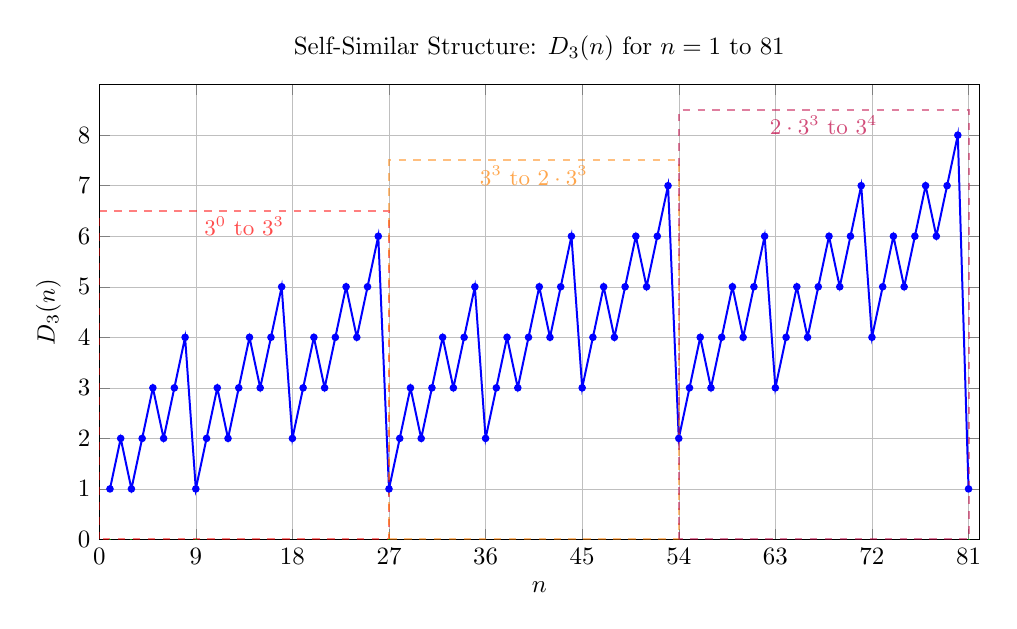
\begin{tikzpicture}[scale=0.9]
\begin{axis}[
    width=14cm,
    height=8cm,
    xlabel={$n$},
    ylabel={$D_3(n)$},
    title={Self-Similar Structure: $D_3(n)$ for $n = 1$ to $81$},
    xmin=0, xmax=82,
    ymin=0, ymax=9,
    xtick={0,9,18,27,36,45,54,63,72,81},
    ytick={0,1,2,3,4,5,6,7,8},
    grid=both,
    grid style={line width=.1pt, draw=gray!10},
    major grid style={line width=.2pt,draw=gray!50},
    legend pos=north west,
]

% Plot D_3(n) --- EXACT values, n = 1..81.
% Corrected 2026-10-31. This block previously held a hand-rolled modular
% expression whose own comment conceded it only "approximated" D_3(n). Evaluated
% against the real base-3 digit sum it disagreed at 72 of these 81 points,
% returning 3 at n=9 and 9 at n=27 where D_3(9) = D_3(27) = 1 --- thereby
% contradicting this figure's own caption ("resets to low values" at the powers
% of 3) and the chapter's own row table. The coordinates below are the base-3
% digit sums themselves.
\addplot[
    color=blue,
    thick,
    mark=*,
    mark size=1.1pt,
] coordinates {(1,1) (2,2) (3,1) (4,2) (5,3) (6,2) (7,3) (8,4) (9,1) (10,2) (11,3) (12,2) (13,3) (14,4) (15,3) (16,4) (17,5) (18,2) (19,3) (20,4) (21,3) (22,4) (23,5) (24,4) (25,5) (26,6) (27,1) (28,2) (29,3) (30,2) (31,3) (32,4) (33,3) (34,4) (35,5) (36,2) (37,3) (38,4) (39,3) (40,4) (41,5) (42,4) (43,5) (44,6) (45,3) (46,4) (47,5) (48,4) (49,5) (50,6) (51,5) (52,6) (53,7) (54,2) (55,3) (56,4) (57,3) (58,4) (59,5) (60,4) (61,5) (62,6) (63,3) (64,4) (65,5) (66,4) (67,5) (68,6) (69,5) (70,6) (71,7) (72,4) (73,5) (74,6) (75,5) (76,6) (77,7) (78,6) (79,7) (80,8) (81,1)};

% Highlight the three main power-of-3 blocks
% Block maxima corrected 2026-10-31 from (5, 7, 9) to the true (6, 7, 8):
% the first rectangle did not enclose its own data and the third overshot.
\draw[red, thick, dashed, opacity=0.5] (axis cs:0,0) rectangle (axis cs:27,6.5);
\node[red, font=\small, opacity=0.7] at (axis cs:13.5,6.2) {$3^0$ to $3^3$};

\draw[orange, thick, dashed, opacity=0.5] (axis cs:27,0) rectangle (axis cs:54,7.5);
\node[orange, font=\small, opacity=0.7] at (axis cs:40.5,7.2) {$3^3$ to $2 \cdot 3^3$};

\draw[purple, thick, dashed, opacity=0.5] (axis cs:54,0) rectangle (axis cs:81,8.5);
\node[purple, font=\small, opacity=0.7] at (axis cs:67.5,8.2) {$2 \cdot 3^3$ to $3^4$};

% Mark powers of 3
\draw[thick, green!50!black] (axis cs:1,0) -- (axis cs:1,-0.3);
\node[below, font=\tiny, green!50!black] at (axis cs:1,-0.4) {$3^0$};

\draw[thick, green!50!black] (axis cs:3,0) -- (axis cs:3,-0.3);
\node[below, font=\tiny, green!50!black] at (axis cs:3,-0.4) {$3^1$};

\draw[thick, green!50!black] (axis cs:9,0) -- (axis cs:9,-0.3);
\node[below, font=\tiny, green!50!black] at (axis cs:9,-0.4) {$3^2$};

\draw[thick, green!50!black] (axis cs:27,0) -- (axis cs:27,-0.3);
\node[below, font=\tiny, green!50!black] at (axis cs:27,-0.4) {$3^3$};

\draw[thick, green!50!black] (axis cs:81,0) -- (axis cs:81,-0.3);
\node[below, font=\tiny, green!50!black] at (axis cs:81,-0.4) {$3^4$};

\end{axis}
\end{tikzpicture}
